\section{Laser reflectance as side information}

\label{sec:modality_ref}
\begin{figure}
	\center
	\begin{minipage}{0.15\linewidth}
		\center\scriptsize
		Images
	\end{minipage}\hfill
	\begin{minipage}{0.84\linewidth}
	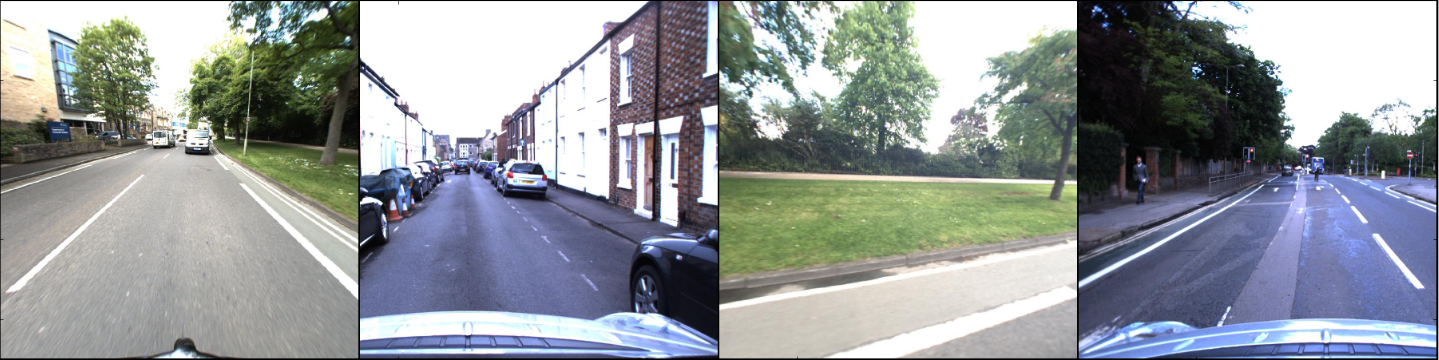
\includegraphics[width=\linewidth]{reflectance/ref_exs/im_1}		
	\end{minipage}
	
	\begin{minipage}{0.15\linewidth}
		\center\scriptsize
		Ground truth reflectance map
	\end{minipage}\hfill
	\begin{minipage}{0.84\linewidth}
	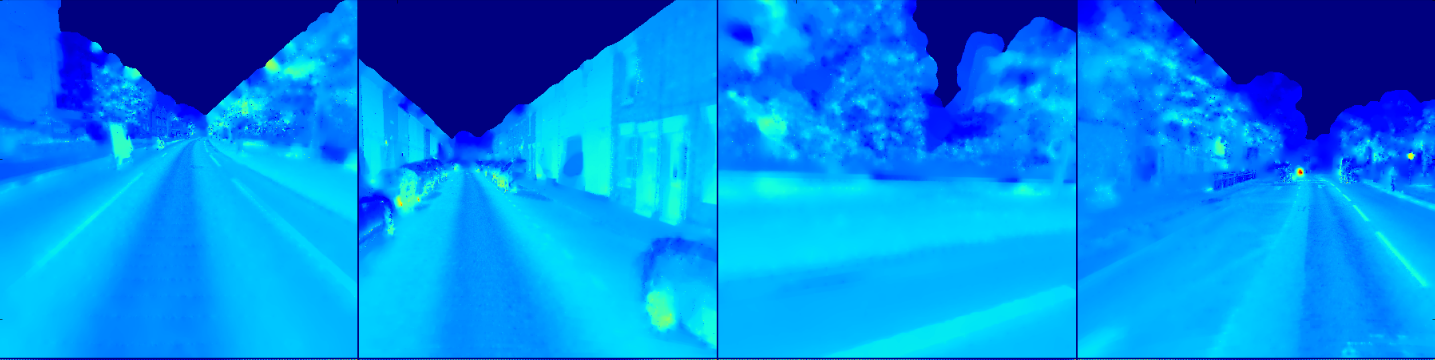
\includegraphics[width=\linewidth]{reflectance/ref_exs/gt_1}	
	\end{minipage}
	
	\begin{minipage}{0.15\linewidth}
		\center\scriptsize		
		Generated reflectance map
	\end{minipage}\hfill
	\begin{minipage}{0.84\linewidth}
	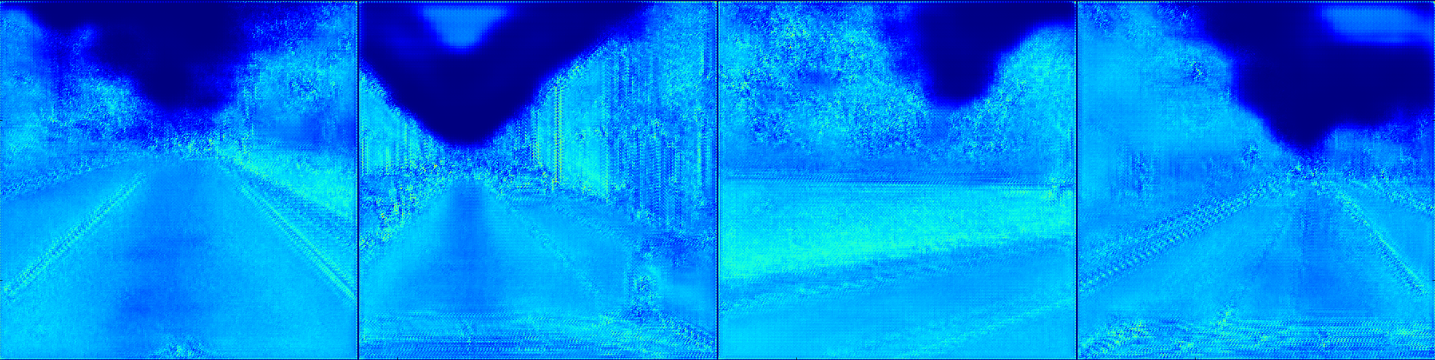
\includegraphics[width=\linewidth]{reflectance/ref_exs/gene_1}	
	\end{minipage}
	
	\caption{\label{fig:ref_examples} \textbf{Examples of dense reflectance map:} the lighter the color, the higher the reflection of the material. Reflectance map highlights reflective areas, like road marking, road sign, vegetation and cars. Figure best viewed in colors.}
\end{figure}

In this section we investigate the use of another modality replacing the depth map in order to evaluate the generalization capabilities of the proposed framework. We use lidar reflectance values as auxiliary modality for these experiments.

\subsection{Laser reflectance}
Lidar reflectance is defined by the proportion of the signal returned to the laser sensor after hitting an object in the scene. Reflectance characterizes the material property of an object. We use the reflectance information provided in the Robotcar dataset~\cite{Maddern2016}. Reflectance value range from 0 to 1 depending if the object as reflected from 0 to 100\% of the original laser beam. We proceed the sparse reflectance data as same as the depth map using inpainting algorithm from~\cite{Bevilacqua2017} to produce dense reflectance maps. We use exactly the same decoder architecture for the reflectance map and the depth map. Examples of dense reflectance map are presented in figure~\ref{fig:ref_examples}.

\subsection{Reflectance versus Depth}
We report in figure~\ref{fig:ref_vs_depth} results using reflectance map during the descriptor training (\textbf{RGB(R)}, in gray). Localization accuracy is slightly worst when using the reflectance map than the results obtained while using the depth map. Still, reflectance information is beneficial as it increase the results over the RGB only descriptor. We can draw the conclusion that scene geometry is more informative for long term localization than reflectance property of observed objects.


\subsection{Multi-modal complementarity}
In this final experiment we compare the performances of a single side modality training descriptor and a multiple side modalities training descriptor. We slightly modify our original system to benefit for both depth and reflectance information. The modified network is presented in figure~\ref{fig:multi_mod}. We report localization results of the three methods, depth map as side information (RGB(D), in blue), reflectance map as side information (RGB(R), in gray) and depth and reflectance map as side information (RGB(DR), in black), in figure~\ref{fig:ref_vs_depth}.

We do not observe systematic improvement when using both modalities. Nevertheless we obtain our best localization results for 3 out of 5 query sets (figure~\ref{fig:ref_vs_depth} b, c \& e). We observe that modality combination is beneficial only if each modal information perform equivalently when used standalone. In other world, if one modality is a lot more informative than the over on a specific dataset (for instance depth over reflectance for the query set CMU - Snow, figure~\ref{fig:ref_vs_depth}-d), the combination of the both will cancel potential benefit given by the most informative modality.

This preliminary results are encouraging concerning the use of multiple modalities during the training process of the descriptor. Still, complementary experiment have to be done, in particular concerning the final descriptor fusion. Modality-aware aggregation descriptor or more complex attention mechanism may be considered~\cite{Seymour2018}.

\begin{figure}
	\center
	\begin{minipage}{0.19\linewidth}
		\center \scriptsize
		\includegraphics[width=\linewidth]{plot/depth_vs_ref/Results_lt_queries/distance}	
		
		\includegraphics[width=\linewidth]{plot/depth_vs_ref/Results_lt_queries/recall}
		
		a) Oxford -- LT
	\end{minipage}
	\begin{minipage}{0.19\linewidth}
		\center \scriptsize
		\includegraphics[width=\linewidth]{plot/depth_vs_ref/Results_snow_queries/distance}	
		
		\includegraphics[width=\linewidth]{plot/depth_vs_ref/Results_snow_queries/recall}
				
		b) Oxford -- Snow
	\end{minipage}
	\begin{minipage}{0.19\linewidth}
		\center \scriptsize
		\includegraphics[width=\linewidth]{plot/depth_vs_ref/Results_cmu_lt/distance}	
		
		\includegraphics[width=\linewidth]{plot/depth_vs_ref/Results_cmu_lt/recall}
		
		c) CMU -- LT
	\end{minipage}
	\begin{minipage}{0.19\linewidth}
		\center \scriptsize
		\includegraphics[width=\linewidth]{plot/depth_vs_ref/Results_cmu_snow/distance}	
		
		\includegraphics[width=\linewidth]{plot/depth_vs_ref/Results_cmu_snow/recall}
		
		d) CMU -- Snow
	\end{minipage}
	\begin{minipage}{0.19\linewidth}
		\center \scriptsize
		\includegraphics[width=\linewidth]{plot/depth_vs_ref/Results_cmu_autumn/distance}	
		
		\includegraphics[width=\linewidth]{plot/depth_vs_ref/Results_cmu_autumn/recall}
		
		e) CMU -- Autumn
	\end{minipage}
	
	\vspace{0.2cm}
	
	\begin{scriptsize}
	\begin{tabular}{c l c l c l }

		\textcolor{blue}{\Large{- -}} & Resnet RGB(D) & 
		\textcolor{gray}{\Large{- -}} & Resnet RGB(R) & 
		\Large{- -} & Resnet RGB(DR) \\
		\textcolor{blue}{\textbf{\Large{---}}} & Alexnet RGB(D) & 
		\textcolor{gray}{\textbf{\Large{---}}} & Alexnet RGB(R) &
		\textbf{\Large{---}} & Alexnet RGB(DR) \\
	\end{tabular}		
	\end{scriptsize}

	\caption[Comparison of depth map and reflectance map as side information]{\label{fig:ref_vs_depth} \textbf{Comparison of depth map and reflectance map as side information.} The geometric information (\textcolor{blue}{in blue}) remains more informative than the reflectance map (\textcolor{gray}{in gray}) for the task of image description for localization. However, when combined (in black), depth map and reflectance map can benefit from each other and produce the most discriminative image descriptors for scenarios b, c \& e. Curves best viewed in colors.}
\end{figure}
\begin{figure}
	\centering
	
	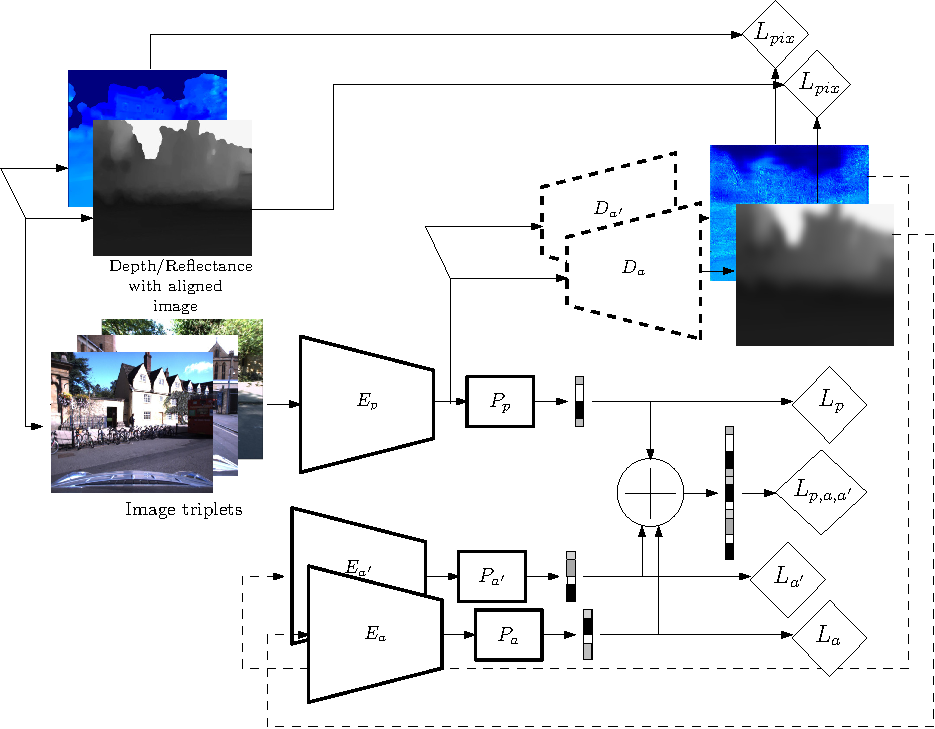
\includegraphics[width=\linewidth]{reflectance/multimod_training}
	
	\caption[Multi-modal training pipeline]{\label{fig:multi_mod} \textbf{Multi-modal training:} we modify the training policy presented in figure~\ref{fig:our_method_deployment} to handle multi-modality. Each generative modal branch ($D_G$ and $D_{Gr}$) can be trained separately. Modality descriptors are trained jointly through the final triplet loss $L_{F_{\theta_D,\theta_R,\theta_I}}$.}
	
\end{figure}